%%%%%%%%%%%%%%%%%%%%%%%%%%%%%%%%%%%%%%%%%%%%%%%%%%%%%%%%%%%%%%%%%%%%%%%%%%%%%%%%%%%%%%
% Modelo de relatório de Disciplina de MLP a partir da
% classe latex iiufrgs disponivel em http://github.com/schnorr/iiufrgs
%%%%%%%%%%%%%%%%%%%%%%%%%%%%%%%%%%%%%%%%%%%%%%%%%%%%%%%%%%%%%%%%%%%%%%%%%%%%%%%%%%%%%%

%%%%%%%%%%%%%%%%%%%%%%%%%%%%%%%%%%%%%%%%%%%%%%%%%%%%%%%%%%%%%%%%%%%%%%%%%%%%%%%%%%%%%%
% Definição do tipo / classe de documento e estilo usado
%%%%%%%%%%%%%%%%%%%%%%%%%%%%%%%%%%%%%%%%%%%%%%%%%%%%%%%%%%%%%%%%%%%%%%%%%%%%%%%%%%%%%%
%
\documentclass[rel_mlp]{iiufrgs}

%%%%%%%%%%%%%%%%%%%%%%%%%%%%%%%%%%%%%%%%%%%%%%%%%%%%%%%%%%%%%%%%%%%%%%%%%%%%%%%%%%%%%%
% Importação de pacotes
%%%%%%%%%%%%%%%%%%%%%%%%%%%%%%%%%%%%%%%%%%%%%%%%%%%%%%%%%%%%%%%%%%%%%%%%%%%%%%%%%%%%%%
% (a A seguir podem ser importados os pacotes necessários para o documento, de acordo
% com a necessidade)
%
\usepackage[brazilian]{babel}	    % para texto escrito em pt-br
\usepackage[utf8]{inputenc}         % pacote para acentuação
\usepackage{graphicx}         	    % pacote para importar figuras
\usepackage[T1]{fontenc}            % pacote para conj. de caracteres correto
\usepackage{times}                  % pacote para usar fonte Adobe Times
\usepackage{enumerate}              % para lista de itens com letras
\usepackage{breakcites}
\usepackage{titlesec}
\usepackage{enumitem}
\usepackage{titletoc}
\usepackage{listings}			    % para listagens de código-fonte
\usepackage{mathptmx}               % p/ usar fonte Adobe Times nas formulas matematicas
\usepackage{url}                    % para formatar URLs
%\usepackage{color}				    % para imagens e outras coisas coloridas
%\usepackage{fixltx2e}              % para subscript
%\usepackage{amsmath}               % para \epsilon e matemática
%\usepackage{amsfonts}
%\usepackage{setspace}			    % para mudar espaçamento dos parágrafos
%\usepackage[table,xcdraw]{xcolor}  % para tabelas coloridas
%\usepackage{longtable}             % para tabelas compridas (mais de uma página)
%\usepackage{float}
%\usepackage{booktabs}
%\usepackage{tabularx}
\usepackage{hyperref}

\usepackage[alf,abnt-emphasize=bf]{abntex2cite}	% pacote para usar citações abnt

% isso meio que coloca helvetica no título dos capítulos, mas fica com muito espaçamento
%\titleformat{\chapter}
%  {\normalfont\fontsize{12}{0}\sffamily\bfseries}
%  {\thechapter}
%  {1em}
%  {}


% isso muda a fonte de tudo:
% \renewcommand\familydefault{\sfdefault}
\newcommand\tab[1][1cm]{\hspace*{#1}}

%%%%%%%%%%%%%%%%%%%%%%%%%%%%%%%%%%%%%%%%%%%%%%%%%%%%%%%%%%%%%%%%%%%%%%%%%%%%%%%%%%%%%%
% Macros, ajustes e definições
%%%%%%%%%%%%%%%%%%%%%%%%%%%%%%%%%%%%%%%%%%%%%%%%%%%%%%%%%%%%%%%%%%%%%%%%%%%%%%%%%%%%%%
%

% define estilo de parágrafo para citação longa direta:
\newenvironment{citacao}{
    %\singlespacing
    %\footnotesize
    \small
    \begin{list}{}{
        \setlength{\leftmargin}{4.0cm}
        \setstretch{1}
        \setlength{\topsep}{1.2cm}
        \setlength{\listparindent}{\parindent}
    }
    \item[]}{\end{list}
}

% adiciona a fonte em figuras e tabelas
\newcommand{\fonte}[1]{\\Fonte: {#1}}

% Ative o seguinte caso alguma nota de rodapé fique muito longa e quebre entre múltiplas
% páginas
%\interfootnotelinepenalty=10000

%%%%%%%%%%%%%%%%%%%%%%%%%%%%%%%%%%%%%%%%%%%%%%%%%%%%%%%%%%%%%%%%%%%%%%%%%%%%%%%%%%%%%%
% Informações gerais
%%%%%%%%%%%%%%%%%%%%%%%%%%%%%%%%%%%%%%%%%%%%%%%%%%%%%%%%%%%%%%%%%%%%%%%%%%%%%%%%%%%%%%

% título
\title{Implementação de um Tower Defense em Swift - Entrega final}

% autor
%\author{Autor2}{Aluno} % {sobrenome}{nome} 1 para cada aluno
\author{Boranga}{Augusto} % {sobrenome}{nome}
\author{Franzoi Scroferneker}{Rodrigo} % {sobrenome}{nome}

% Professor orientador da disciplina
\advisor[Prof.~Dr.]{Mello Schnorr}{Lucas}

% Nome do(s) curso(s):
\course{Curso de Graduação em Ciência da Computa{\c{c}}{\~a}o e Engenharia de Computação}

% local da realização do trabalho
\location{Porto Alegre}{RS}

% data da entrega do trabalho (mês e ano)
\date{12}{2017}


% Palavras chave
\keyword{Palavra-chave1}
\keyword{Palavra-chave2}
\keyword{Palavra-chave3}

%%%%%%%%%%%%%%%%%%%%%%%%%%%%%%%%%%%%%%%%%%%%%%%%%%%%%%%%%%%%%%%%%%%%%%%%%%%%%%%%%%%%%%
% Início do documento e elementos pré-textuais
%%%%%%%%%%%%%%%%%%%%%%%%%%%%%%%%%%%%%%%%%%%%%%%%%%%%%%%%%%%%%%%%%%%%%%%%%%%%%%%%%%%%%%

% Declara início do documento
\begin{document}

% inclui folha de rosto
\maketitle

\selectlanguage{brazilian}

% Declarar aqui todas as referências
\nocite{tower_defense}
\nocite{best_tower_defense}
\nocite{swift}
\nocite{why_learn_swift}
\nocite{o_que_e_paradigma}
\nocite{how_to_use_bibtex}
\nocite{functional_swift_fold_it_baby}
\nocite{an_introduction_to_functional_programming_in_swift}
\nocite{swift_apple_developer_functions}
\nocite{intro_to_swift_functional_programming_with_bob}
\nocite{geison_medium_functional_swift}
\nocite{catp_01}
\nocite{swift_history}


% Sumario
\tableofcontents

%%%%%%%%%%%%%%%%%%%%%%%%%%%%%%%%%%%%%%%%%%%%%%%%%%%%%%%%%%%%%%%%%%%%%%%%%%%%%%%%%%%%%
% Aqui comeca o texto propriamente dito
%%%%%%%%%%%%%%%%%%%%%%%%%%%%%%%%%%%%%%%%%%%%%%%%%%%%%%%%%%%%%%%%%%%%%%%%%%%%%%%%%%%%%

%espaçamento entre parágrafos
%\setlength{\parskip}{6 pt}

\selectlanguage{brazilian}



%%%%%%%%%%%%%%%%%%%%%%%%%%%%%%%%%%%%%%%%%%%%%%%%%%%%%%%%%%%%%%%%%%%%%%%%%%%%%%%%%%%%%
% Intro
%

\chapter{INTRODUÇÃO} \label{intro}

Este relatório discorre sobre o trabalho final da disciplina de Modelos de Linguagem de Programação, explicando as decisões tomadas e os requisitos cumpridos ao longo do desenvolvimento.

O objetivo deste trabalho é implementar um problema computacional em dois paradigmas diferentes (Orientação a Objetos e Funcional) utilizando uma mesma linguagem.

Escolhemos implementar um jogo do gênero Tower Defense com a linguagem Swift.

% REMOVER CITACAO ACIMA

Nosso código-fonte encontra-se no seguinte repositório:
\texttt{\\\tab https://github.com/gutoboranga/tower-defense}

%%%%%%%%%%%%%%%%%%%%%%%%%%%%%%%%%%%%%%%%%%%%%%%%%%%%%%%%%%%%%%%%%%%%%%%%%%%%%%%%%%%%%
% Problema
%

\chapter{PROBLEMA} \label{intro}

Escolhemos para implementar o problema do jogo Tower Defense.

Tower Defense é um subgênero de jogos de estratégia, onde o jogador deve defender seu território (que varia de acordo com a temática do jogo) contra o ataque de inimigos, podendo utilizar um montante inicial para adquirir elementos do jogo que o ajudem na defesa.


%%%%%%%%%% Seção 1

\section{Dinâmica do jogo}

Basicamente, há dois elementos essenciais em um jogo do estilo Tower Defense:

\begin{itemize}[leftmargin=3em]
\setlength{\itemindent}{1em}

    \item Territórios ou propriedades com certa quantidade de vida (o esgotamento desta implica em fim de jogo), que o jogador deve defender;

    \item Inimigos (com outra quantidade de vida) atacando os territórios do jogador;

\end{itemize}

A dinâmica do jogo com estes elementos é de que há "ondas" de ataques dos inimigos ao jogador. Isto é, o ataque ocorre em partes, com pequenas pausas entre eles.

O jogador pode então, entre ou durante as ondas de ataques (isto varia de jogo para jogo), utilizar-se de subterfúgios que atrapalhem a missão dos inimigos (como por exemplo, posicionar obstáculos ou outras estruturas que os ataquem). A aquisição destes equipamentos de defesa custa um certo valor que é decrementado do montante disponível para o jogador.

O objetivo do jogador é sobreviver ao final das N ondas de ataques inimigos.


\section{Historicamente}

Os primeiros jogos de Tower Defense datam da década de 1980, considerada a Era de Ouro dos video-games.

No jogo \textit{Space Invaders} - um clássico dos video-games lançado em 1978 -, o jogador deve defender seu território atirando em invasores alienígenas. É tido por uns como um precursor dos jogos de Tower Defense, mas isto é contestado por outros pelo fato de não possuir um elemento fundamental do gênero: a possibilidade de aquisição de elementos extras que auxiliem o jogador na defesa.

Já o jogo \textit{Rampart} - lançado em 1990 -, é amplamente considerado como o jogo que definiu o gênero, por possuir todos os elementos fundamentais deste. Em \textit{Rampart}, as fases de preparação (posicionamento dos itens de defesa), ação (momento em que a base é atacada e o jogador deve defendê-la) e reparação (consertar elementos danificados pelos ataques) são bem distintas.

\begin{figure}[htb]
    \centering
    \caption{Space Invaders, um dos pioneiros}
    \fbox{
        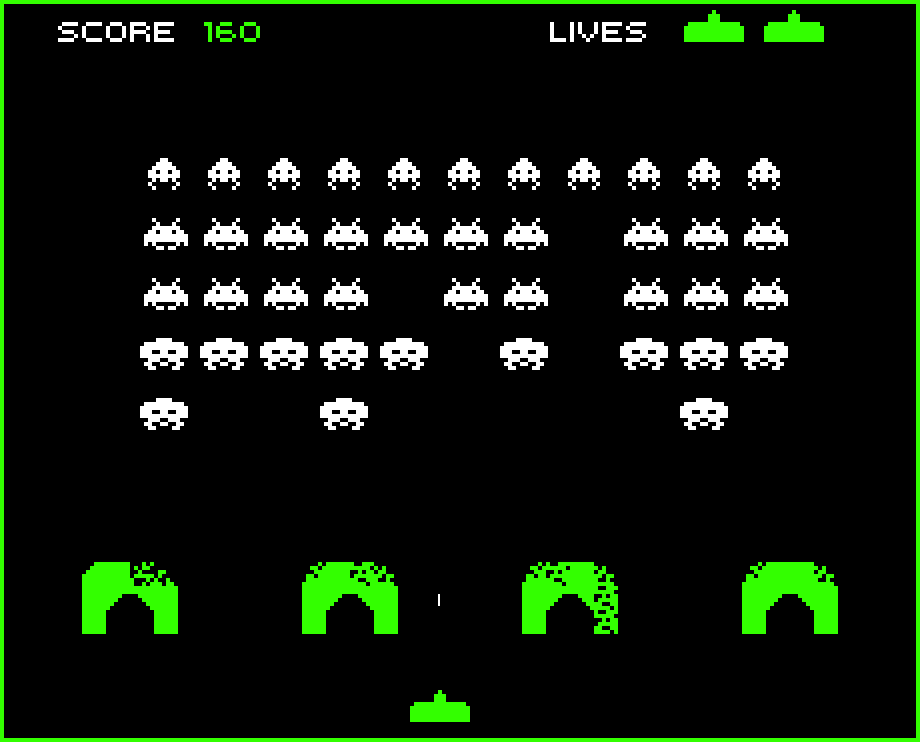
\includegraphics[width=12cm,height=8cm,keepaspectratio]{images/space-invaders.png}
    }
    \label{fig:figura1}
    \fonte{http://fantendo.wikia.com/wiki/File:Space-Invaders.png}
\end{figure}

\begin{figure}[htb]
    \centering
    \caption{Rampart, o Tower Defense clássico}
    \fbox{
        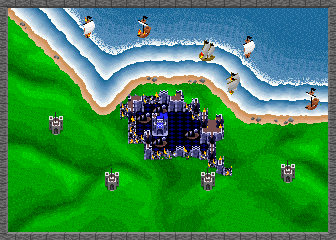
\includegraphics[width=12cm,height=8cm,keepaspectratio]{images/rampart.png}
    }
    \label{fig:figura2}
    \fonte{http://www.wikiwand.com/en/Rampart\_(video\_game)}
\end{figure}


%%%%%%%%%%%%%%%%%%%%%%%%%%%%%%%%%%%%%%%%%%%%%%%%%%%%%%%%%%%%%%%%%%%%%%%%%%%%%%%%%%%%%
% Linguagem
%

\chapter{LINGUAGEM} \label{intro}

Swift é uma linguagem de programação multiparadigma que se apresenta como uma linguagem moderna e focada em três aspectos: segurança, performance e suporte à aplicação de design patterns.

Mesmo sendo consideravelmente recente, Swift demonstra uma comunidade de bom tamanho, ficando em 11º nas linguagens mais populares e a 4ª mais amada no site stackoverflow em 2017.

Neste capítulo daremos um panorama a respeito da linguagem adotada, explanando acerca de suas origens e discutindo seus pontos positivos e negativos.


\section{História}

Swift é uma das linguagens de programação mais recentes desenvolvidas no mercado. Foi apresentada em 2014 na WWDC (Worldwide Developers Conference, evento organizado pela Apple para divulgação de novos produtos e features).

Baseada e influenciada por Objective-C, Ruby e Python, se mostrou uma linguagem poderosa e de fácil compreensão (devido principalmente, à sua sintaxe simples).

Inicialmente, Swift era de uso exclusivo por usuários de Mac OS, visto que este era o único sistema operacional habilitado a compilar a linguagem. Em dezembro de 2015, porém, um grande anúncio mudou o jogo: Swift viraria open source, abrindo um leque ainda maior de possibilidades de uso para a linguagem. \cite{swift_history}


\section{Aspectos técnicos}

Swift é uma linguagem multiparadigma, suportando programação funcional e também oferecendo recursos de Orientação a Objetos, como classes e protocolos.

A linguagem possui tipagem estática, o que proporciona maior segurança (garantia dos tipos de dados esperados no código, evitando erros de tipos) e performance (não há gasto de máquina com checagem dos tipos) às aplicações que a utilizam.

Por ter sido construída pela Apple, possui alta integração com Obj-C, outra linguagem utilizada no ambiente da Apple. Assim sendo, o programador que utiliza Swift tem à sua disposição uma série de bibliotecas em Obj-C, como por exemplo \textit{SpriteKit}, a biblioteca de construção de jogos que utilizaremos no desenvolvimento do trabalho.

Sua sintaxe foi pensada para ser o mais simples e expressiva possível, tornando o código mais fácil de ler e escrever. \cite{why_learn_swift}


\section{Utilização}

Mesmo sendo uma linguagem relativamente recente, Swift agradou a comunidade de desenvolvimento. Na pesquisa do site stackoverflow realizada em 2017, Swift ficou em 4º lugar nas linguagens preferidas pelos usuários.

Suas principais aplicações são:

\begin{itemize}[leftmargin=3em] % [label={--}]
\setlength{\itemindent}{1em}

    \item \textbf{Mobile}: Swift é a linguagem oficial para desenvolvimento de aplicativos para a plataforma iOS. Obj-C também é suportada em iOS, mas o programador mobile é encorajado pela própria Apple a utilizar Swift por esta ser uma linguagem mais recente e simples de usar;

    \item \textbf{Desktop}: Similar à plataforma mobile (citada acima), aplicações para o sistema operacional dos computadores da Apple (macOS, antigamente chamado OS X) também podem ser escritas em Swift;

    \item \textbf{Servidor}: Além disso, Swift também pode ser utilizado para o desenvolvimento de aplicações no lado do servidor. Existem alguns frameworks e toolkits (como o Perfect) que auxiliam o desenvolvedor nesta tarefa.

\end{itemize}

\section{Motivo da escolha}

Optamos por Swift por dois motivos:

\begin{itemize}[leftmargin=3em]
\setlength{\itemindent}{1em}

    \item Ambos os integrantes do grupo tem familiaridade com a linguagem, devido a experiência prévia desenvolvendo aplicativos mobile.

    \item Swift é uma linguagem muito intuitiva e possui uma variedade de bibliotecas auxiliares disponíveis.

\end{itemize}

\section{Análise}

Ao término do trabalho estamos habilitados para fazer uma análise mais técnica da linguagem. Para isto, usaremos as características presentes no Formulário de Avaliação de Linguagens \cite{catp_01}.

\subsection{Simplicidade}

Nota: 8/10

Consideramos Swift uma linguagem com sintaxe bem simples e fácil de aprender.

\subsection{Ortogonalidade}

Nota: X/10

TODO

\subsection{Estrutura de Controle}

Nota: 6/10

TODO

\subsection{Tipos de Dados}

Nota: 10/10

A linguagem tem suporte à criação de diversos tipos de dados como classes e enumerações.

\subsection{Estruturas de Dados}

Nota: 9/10

TODO:

\subsection{Suporte a Abstração de Dados}

Nota: 9/10

TODO:

\subsection{Suporte a Abstração de Controle}

Nota: 8/10

TODO:

\subsection{Expressividade}

Nota: 9/10

Swift é uma linguagem bastante expressiva. Isto é, poucos comandos em Swift representam muitos comandos em linguagem de máquina.

\subsection{Checagem de Tipos}

Nota: 8/10

Swift é uma linguagem compilada com checagem de tipos.

\subsection{Restrições de Aliasing}

Nota: ?

TODO

\subsection{Suporte ao Tratamento de Exceções}

Nota: 8/10

O tratamento de exceções é bem simples e prático de ser implementado em Swift.

\subsection{Portabilidade}

Nota: 6/10

A linguagem tornou-se \textit{open source} há pouco tempo. Portanto, a portabilidade aumentou bastante de lá pra cá. Entretanto, seu maior uso ainda é em sistemas fechados, como o desenvolvimento para plataformas proprietárias: iOS, macOS e watchOS (todos da Apple), por exemplo.

\subsection{Reusabilidade}

Nota: 7/10

A linguagem permite a criação de frameworks, que podem ser distribuídos através de gerenciadores de dependências (como o \textit{Cocoa Pods}, por exemplo). Isto promove a reusabilidade de projetos em Swift.

\subsection{Tamanho de Código}

Nota: 9/10

A linguagem permite expressar muitas ações em poucas linhas de código, se comparada com funções correspondentes em C ou Objective-C.



%%%%%%%%%%%%%%%%%%%%%%%%%%%%%%%%%%%%%%%%%%%%%%%%%%%%%%%%%%%%%%%%%%%%%%%%%%%%%%%%%%%%%

\chapter{IMPLEMENTAÇÃO} \label{intro}

\section{Paradigma Orientado a Objetos} \label{intro}

Na primeira etapa do trabalho, optamos por implementar o jogo usando Orientação a Objetos devido a conhecimento prévio de ambos integrantes do grupo.

Acreditamos que será mais fácil implementar o jogo no paradigma funcional como segunda etapa ao invés da primeira, pois agora temos um conhecimento maior acerca da linguagem e das regras do próprio jogo.

\subsection{Requisitos}

A seguir está a lista de requisitos para o paradigma de Orientação a Objetos. Para cada requisito cumprido na implementação, há um exemplo retirado do nosso código-fonte.

\subsubsection{Classes}

Especificar e utilizar classes (utilitárias ou para representar as estruturas de dados utilizadas pelo programa).

Utilizamos diversas classes no projeto inteiro, seguindo o padrão MVC com leves alterações devido à presença do conceito de GameScene, trazido pela biblioteca de jogos SpriteKit.

Exemplo: classe \texttt{Projectile}, que representa um projétil atirado pelas torres do jogo.
\texttt{\\class Projectile: StandardBlock \{\\\tab ...\\\}}

%%%%%%%%%%%%%%%%%%%%%

\subsubsection{Encapsulamento}

Fazer uso de encapsulamento e proteção dos atributos, com os devidos métodos de manipulação (setters/getters) ou propriedades de acesso, em especial com validação dos valores (parâmetros) para que estejam dentro do esperado ou gerem exceções caso contrário.

Exemplo:

Praticamos onde possível (e necessária) a proteção dos atributos. Por exemplo, na classe \texttt{LifeBar}, que representa a porcentagem de vida dos personagens do jogo (e seu elemento visual, no formato de uma barra que muda de acordo com o valor associado), há as seguintes funções de get e set.

\texttt{\\public func getLife() -> Double \{\\\tab return self.actualLife\\\}}

\texttt{\\public func setLife(newValue: Double) \{\\\tab self.actualLife = newValue\\\}}
    
O objetivo aqui é proteger o atributo privado \texttt{actualLife}, que representa o quanto de vida o objeto que possui este \texttt{LifeBar} ainda possui dentro do jogo.

%%%%%%%%%%%%%%%%%%%%%

\subsubsection{Construtores-Padrão}

Especificação e uso de construtores-padrão para a inicialização dos atributos e, sempre que possível, de construtores alternativos.

Na maioria das classes implementadas, criamos apenas um construtor - com parâmetros - pois não encontramos necessidade de criar construtores padrão, uma vez que em Swift pode-se inicializar os atributos de uma classe junto com sua declaração. Ao adotar esta prática, os atributos já terão valores default na criação do objeto.

Na classe \texttt{Enemy}, temos um construtor padrão que inicializa os elementos que ainda não haviam sido inicializados na declaração e chamamos o método \texttt{init} da classe pai (super.init(parâmetros)).

%%%%%%%%%%%%%%%%%%%%%

\subsubsection{Destrutores}

Especificação e uso de destrutores (ou métodos de finalização), quando necessário.

Não houve necessidade de criar destrutores nas classes implementadas pois o framework utilizado lida com a desalocação de memória de maneira competente.

%%%%%%%%%%%%%%%%%%%%%

\subsubsection{Espaços de nome}

Organizar o código em espaços de nome diferenciados, conforme a função ou estrutura de cada classe ou módulo de programa.

Não foi implementado.

%%%%%%%%%%%%%%%%%%%%%

\subsubsection{Herança}

Usar mecanismo de herança, em especial com a especificação de pelo menos três níveis de hierarquia, sendo pelo menos um deles correspondente a uma classe abstrata, mais genérica, a ser implementada nas classes-filhas.

Exemplo:

Temos a classe \texttt{StandardBlock}, que é uma classe abstrata da  qual a maioria dos personagens do jogo herda. \texttt{StandardBlock} possui apenas um atributo de orientação no espaço e métodos para manipular este atributo.

Dentre suas herdeiras está a classe \texttt{Enemy}, que representa o tipo genérico de todos os inimigos presentes no jogo. Esta classe possui atributos e métodos comuns a todas as especificações de inimigos.

Por sua vez, \texttt{Enemy} possui algumas classes herdeiras que especializam e personalizam o conceito genérico de inimigo, com implementações específicas de funções genéricas de acordo com as características deste personagem. Por exemplo, temos a classe \texttt{AstronautEnemy}, que representa o personagem astronauta.

%%%%%%%%%%%%%%%%%%%%%

\subsubsection{Polimorfismo por inclusão}

Utilizar polimorfismo por inclusão (variável ou coleção genérica manipulando entidades de classes filhas, chamando métodos ou funções específicas correspondentes).

Como citado anteriormente na seção Herança, temos a classe \texttt{Enemy} representando a classe genérica dos inimigos no jogo. Ela possui alguns métodos que devem ser sobrecarregados pelas suas herdeiras, de acordo com as características destas.

Por exemplo, o método \texttt{getDamageValue()}, que retorna um Double representando o valor do dano que este inimigo causa ao atingir o castelo do jogador. Para a classe \texttt{AstronautEnemy} (que no âmbito do jogo representa um ser humano), esta função é implementada de forma a retornar o valor 0.7, enquanto que na classe \texttt{RoverEnemy} (que representa um veículo de exploração espacial, portanto mais forte do que um ser humano), a implementação desta função retorna o valor 2.0.

%%%%%%%%%%%%%%%%%%%%%

\subsubsection{Polimorfismo paramétrico}

Usar polimorfismo paramétrico através da especificação de \textit{algoritmo} (método ou função genérico) utilizando o recurso oferecido pela linguagem (i.e., generics, templates ou similar) e da especificação de \textit{estrutura de dados} genérica utilizando o recurso oferecido pela linguagem.

Exemplo:

Implementamos uma função que previne erros na física da colisão dos elementos do jogo. Esta função recebe dois parâmetros de qualquer tipo e retorna um booleano que indica se seu tipo (mais genérico) é o mesmo.

\texttt{\\func sameType<T,E>(one : T, two: E) -> Bool \{\\\tab if type(of: one) == type(of: two) \{\\\tab \tab return true\\\tab\}\\\tab return false\\\}}

%func sameType<T,E>(one : T, two: E) -> Bool {
%    if type(of: one) == type(of: two) {
%        return true
%    }
%    return false
%}

%%%%%%%%%%%%%%%%%%%%%

\subsubsection{Polimorfismo por sobrecarga}

Usar polimorfismo por sobrecarga (vale construtores alternativos).

Utilizamos polimorfismo por sobrecarga na classe \texttt{Enemy}, onde temos duas implementações (com assinaturas diferentes) para a função \texttt{move()}:

\begin{itemize}
\setlength{\itemindent}{1em}
    \item Uma delas é pública e não recebe parâmetros, tendo a seguinte assinatura, portanto:
    
    \texttt{public func move()}
    
    Esta serve para iniciar o movimento de um inimigo, e é chamada de fora da classe que a implementa, indicando o início do movimento de um inimigo.
    
    \item A segunda é privada e recebe como parâmetro uma lista de movimentos (pares ordenados x, y) a serem feitos pelo inimigo em questão. Sua assinatura é a seguinte:
    
    \texttt{private func move(\_ newDir : [[CGFloat]])}
    
    Nesta função privada, é realizado o movimento até a primeira posição (x, y) da lista recebida e após, são feitas chamadas recursivas passando como parâmetro a lista sem o primeiro elemento.
\end{itemize}


%- A segunda é privada e recebe como parâmetro uma lista de movimentos pares ordenados (x, y). Sua assinatura é a seguinte::
%private func move(_ newDir : [[CGFloat]])
%Nesta função privada, é realizado o movimento para a primeira posição (x, y) da lista recebida e após, são feitas chamadas recursivas %para ela mesma enviando a lista sem o primeiro elemento.

%%%%%%%%%%%%%%%%%%%%%

\subsubsection{Delegates}

Especificar e usar delegates.

Utilizamos o conceito de delegate (em Swift conhecido como protocol) para fazer a comunicação entre os elementos visuais do jogo (View, no padrão MVC) com a parte mais conceitual (Model) sem criar dependências desnecessárias entre estas classes.

Exemplo:

Na classe \texttt{Tower} (que modela o conceito de uma torre de defesa dentro do jogo), é declarado o seguinte delegate:

\texttt{\\ protocol TowerDelegate \{\\\tab func removeTower(tower : Tower)\\\tab func upgradeTower(tower: Tower)\\\}}

A classe que implementa este delegate é a \texttt{GameScene}. Ela é, portanto, a responsável por tomar as ações necessárias quando a classe \texttt{Tower} acionar algum dos métodos declarados neste protocol. Estas ações envolvem chamadas a métodos de outras classes. O uso deste delegate evita que a classe \texttt{Tower} fique acoplada a estas outras classes, deixando que a \texttt{GameScene} faça a comunicação necessária entre elas.

%%%%%%%%%%%%%%%%%%%%%%%%%%%%%%%%%%%%%%%%%%%%%%%%%%%%%%%%%%%%%%%%%%%%%%%%%%%%%%%%%%%%%
% Funcional
%
\section{Paradigma Funcional}

Na segunda etapa do trabalho, implementamos o jogo utilizando técnicas do paradigma de Programação Funcional. Não fizemos uma implementação completamente funcional devido à algumas limitações do framework utilizado para a criação do jogo, mas sempre que possível aplicamos os mecanismos de programação funcional vistos em aula.

%%%%%%%%%%%%%%%%%%%%%

\subsection{Requisitos}

A seguir estão listados os requisitos para o paradigma funcional. Para cada requisito cumprido na implementação, há um exemplo retirado do nosso código-fonte.

%%%%%%%%%%%%%%%%%%%%%

\subsubsection{Elementos imutáveis e funções puras}

Demos prioridade ao uso de elementos imutáveis sempre que possível. Uma exemplo disto é na manipulação de listas com recursão, em que criamos uma nova instância da lista e a passamos adiante, ao invés de alterar a lista original.

No item \texttt{recursão} abaixo, está o trecho de código completo, mas aqui a chamada recursiva que fazemos enviando como parâmetro um novo array, criado a partir do array atual, mas retirando o primeiro elemento.

\texttt{
\\self.spawnEnemy(Array(enemies.dropFirst()))
}

%%%%%%%%%%%%%%%%%%%%%

\subsubsection{Funções lambda}

Algumas funções que utilizamos recebem como parâmetro um pedaço de código (um \texttt{callback}, ou \texttt{completion}) a ser executado após certa instrução.

Nosso exemplo é a função \texttt{loseLife}, que faz com que um elemento do jogo tenha sua quantidade de vida descrescida em um dado valor, e após, executa o trecho de código recebido por parâmetro.

Declaração da função \texttt{loseLife}:

\texttt{
\\func loseLife(with damage:Double, completion: () -> ()) \{
\\\tab lifeBar.loseLife(with: damage) \{
\\\tab\tab completion()
\\\tab \}
\\\}
}

Exemplo de chamada da função passando uma função anônima por parâmetro:

\texttt{
\\castle.loseLife(with: enemy.getDamageValue(), completion: \{
\\\tab self.removeFromParent()
\\\tab self.gameDelegate?.endOfGame(won: false, score: self.score)
\\\}
}

%%%%%%%%%%%%%%%%%%%%%

\subsubsection{Currying}

Não foi implementado.

%%%%%%%%%%%%%%%%%%%%%

\subsubsection{Pattern matching}

O tipo de pattern-matching que usamos é chamado em Swift \texttt{Value-binding pattern}. Este tipo é, em outras palavras, o uso do mecanismo de \texttt{switch} na asserção de valores possíveis acerca de uma variável ou constante.

\texttt{
\\switch button.name! {
\\\tab case "speed":
\\\tab\tab tower = SpeedTower(size: s, position: p)
\\\tab case "damage":
\\\tab\tab tower = DamageTower(size: s, position: p)
\\\tab case "range":
\\\tab\tab tower = RangeTower(size: s, position: p)
\\\tab default:
\\\tab\tab tower = DoubleShotTower(size: s, position: p)
\\\tab }
\\\}
}

Além disso, utilizamos pattern matching nas \texttt{enumerations}:

\texttt{
\\var title : String \{
\\\tab switch self \{
\\\tab\tab case .won:
\\\tab\tab\tab return "You won!"
\\\tab\tab default:
\\\tab\tab\tab return "Game over"
\\\tab \}
\\\}
}

Aqui, o \texttt{switch} tenta dar match no valor de \texttt{self} (o objeto do tipo do \texttt{enum}) com os possíveis valores (\texttt{won} ou \texttt{lost}, que fica como default) para retornar uma \texttt{String} associada.

%%%%%%%%%%%%%%%%%%%%%

\subsubsection{Funções de ordem superior próprias}

Não foi implementado.

%%%%%%%%%%%%%%%%%%%%%

\subsubsection{Funções de ordem superior prontas}

Utilizamos sempre que possível as funções de ordem superior oferecidas pela linguagem. Alguns exemplos:

Na função que trata o clique do usuário na tela, precisamos descobrir se no ponto x,y clicado há uma torre, para então tomar as devidas providências em caso positivo ou negativo.
Para isto, aplicamos a função \texttt{reduce} (que retorna um valor ao final da iteração sobre a lista) sobre a lista de torres em atividade no momento, de modo a retornar um booleano no final que indica se alguma das torres foi clicada.

\texttt{
\\let foundTower = towers.reduce(false, \{ (hasFoundTowerYet, tower) \tab\tab\tab\tab\tab\tab\tab\tab\tab\tab\tab\tab\tab-> Bool in
    \\\tab if let t = tower as? Tower \{
    \\\tab\tab if t.contains(point) \{
    \\\tab\tab\tab t.mouseDown(with: event)
    \\\tab\tab\tab return hasFoundTowerYet || true
    \\\tab\tab \}
    \\\tab \}
    \\\tab return hasFoundTowerYet || false
\\\})}

No menu final do jogo, há vários botões de ações que podem ser tomadas, entre elas recomeçar o jogo e voltar ao menu inicial.
Para tratar o clique neste menu, precisamos descobrir se ele ocorreu em algum dos nodos (o nodeo é a estrutura básica do framework, para qualquer tipo de representação visual) que podem ser clicados (no caso, nodos de texto, os \texttt{SKLabelNode}). Isto é, precisamos filtrar os nodos que estavam no ponto x,y clicado para pegar apenas os nodos de texto.

\texttt{
\\let labelNodes = allNodes.filter(\{
\\\tab return \$0.isMember(of: SKLabelNode.self)
\\\})}

%%%%%%%%%%%%%%%%%%%%%

\subsubsection{Funções como elementos de 1ª ordem}

A função nodeIsClickable recebe um \texttt{SKNode} (elemento visual mais básico) e retorna um booleano. Serve como um filtro pra saber se será necessário tratar o clique do usuário (se clicou em um nodo que desencadeia uma ação) ou se foi um clique sem consequências.

Implementação da função:

\texttt{
\\func nodeIsClickable(node: SKNode) -> Bool \{
\\\tab return node == self.newGameLabel! ||
\\\tab\tab\tab node == self.quitLabel! ||
\\\tab\tab\tab node == self.mainMenuLabel!
\\\}}
    
Uso com o método \texttt{first(where: f)}, que recebe uma função do tipo \texttt{(SKNode) -> (Bool)} como parâmetro e retorna o primeiro elemento que satisfizer a condição da funcao recebida (ou seja, quando a função retornar true). Aqui referenciamos nossa função definida acima.

\texttt{\\let labelToSelect = labelNodes.first(where: nodeIsClickable)}

%%%%%%%%%%%%%%%%%%%%%

\subsubsection{Recursão}

Utilizamos recursão em alguns momentos em que era necessário manipular listas passando adiante cópias da lista original removendo seus elementos.
Nosso exemplo é da função \texttt{spawnEnemy}, que serve para adicionar os inimigos na tela.

\texttt{
\\func spawnEnemy(\_ enemies: [Int]) \{
\\\tab self.enemiesToSpawn -= 1
\\\tab if let enemyType = enemies.first \{
\\\tab\tab run(SKAction.wait(forDuration: enemiesDelay), completion:
\\\tab\tab \{
\\\tab\tab\tab self.handleEnemyTypes(type: enemyType)
\\\tab\tab\tab self.spawnEnemy(Array(enemies.dropFirst()))
\\\tab\tab \})
\\\tab \}
\\\}
}

%%%%%%%%%%%%%%%%%%%%%%%%%%%%%%%%%%%%%%%%%%%%%%%%%%%%%%%%%%%%%%%%%%%%%%%%%%%%%%%%%%%%%
% Screenshots
%
\chapter{SCREENSHOTS}

A seguir estão listados alguns screenshots tirados durante a execução do nosso jogo.

\begin{figure}[htb]
    \centering
    \caption{Menu inicial}
    \fbox{
        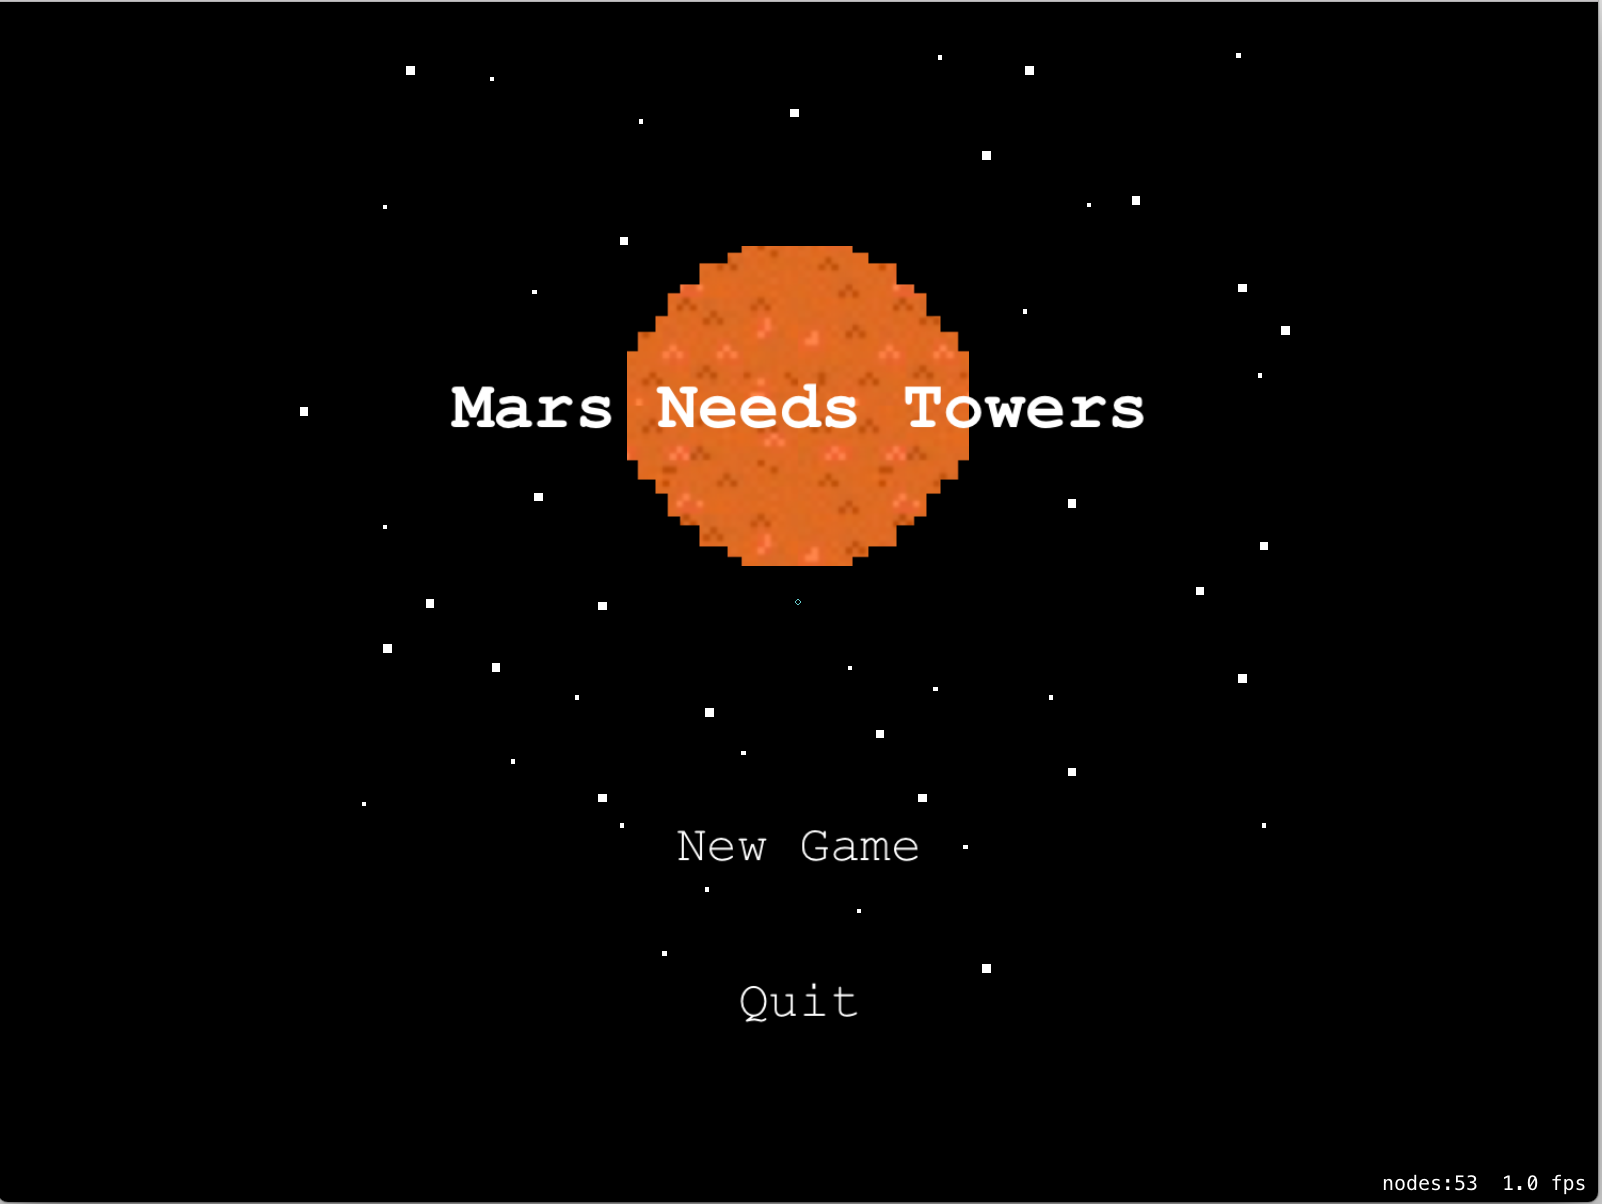
\includegraphics[width=12cm,height=8cm,keepaspectratio]{images/main-menu.png}
    }
    \label{fig:figura1}
\end{figure}

\begin{figure}[htb]
    \centering
    \caption{Jogo em ação}
    \fbox{
        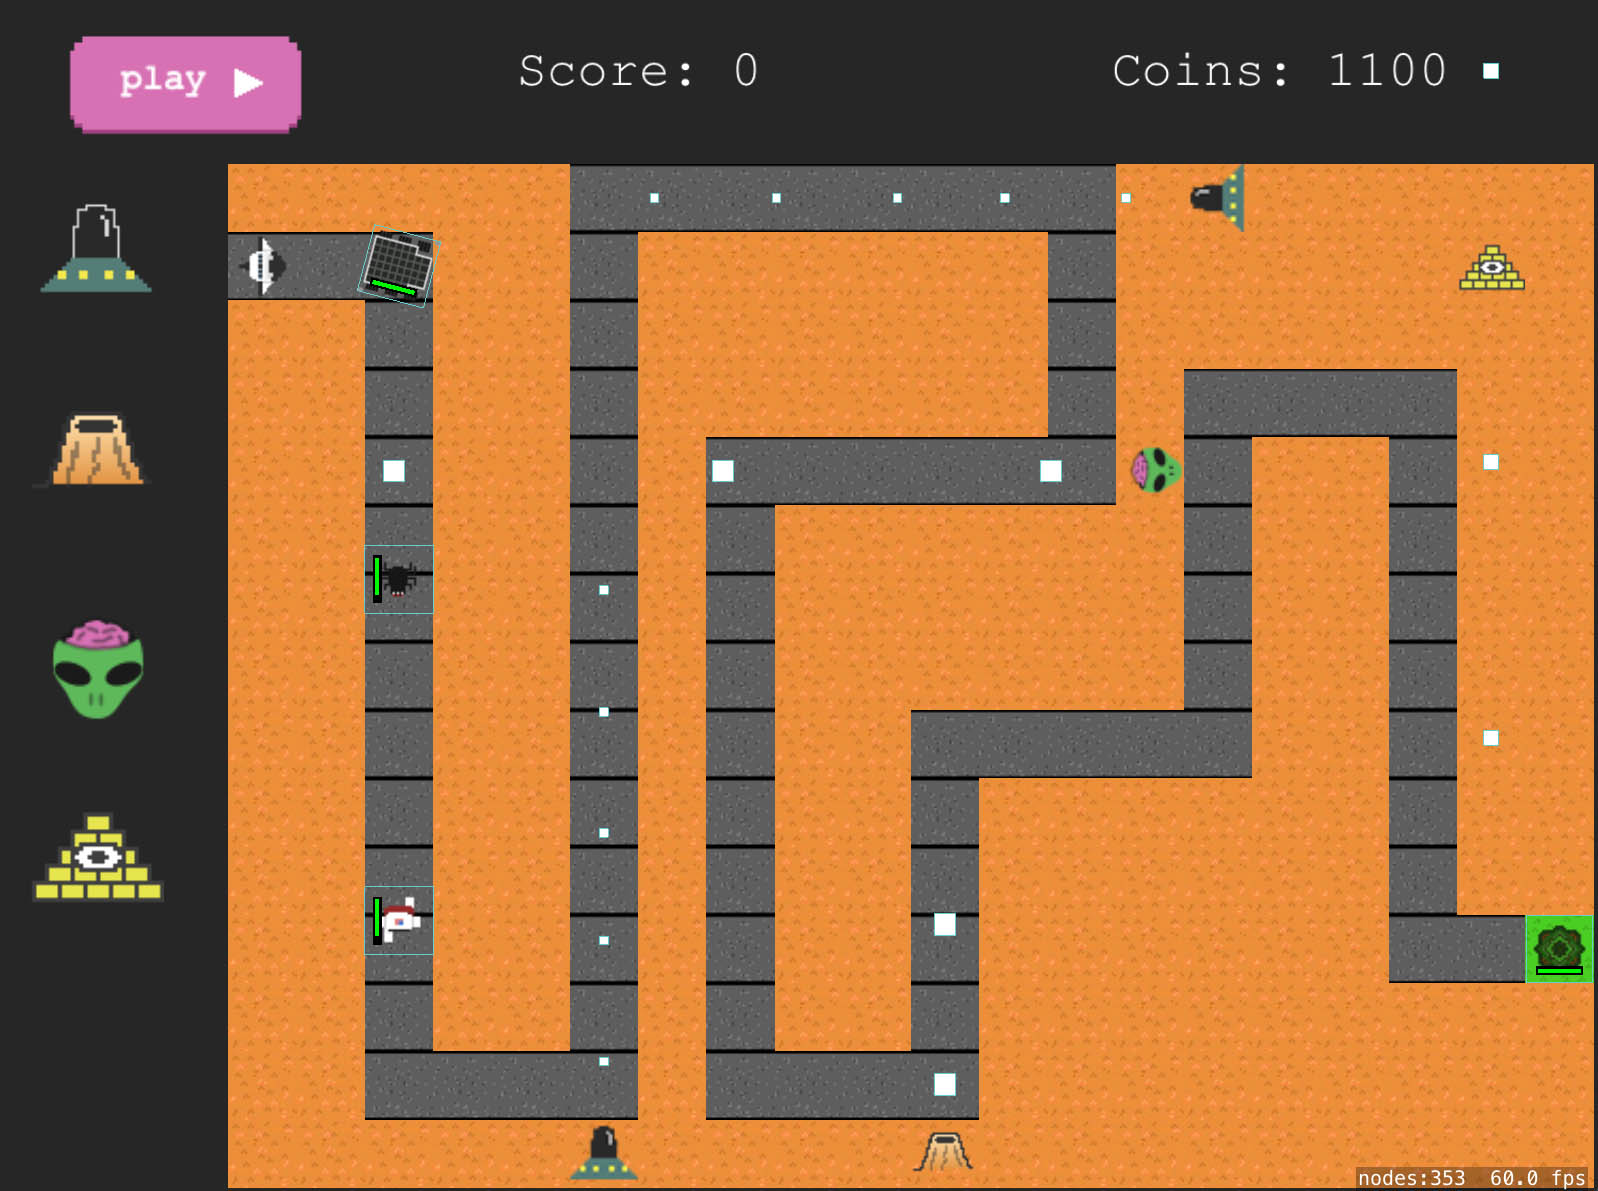
\includegraphics[width=12cm,height=8cm,keepaspectratio]{images/battle.png}
    }
    \label{fig:figura1}
\end{figure}

\begin{figure}[htb]
    \centering
    \caption{Final do jogo: vitória}
    \fbox{
        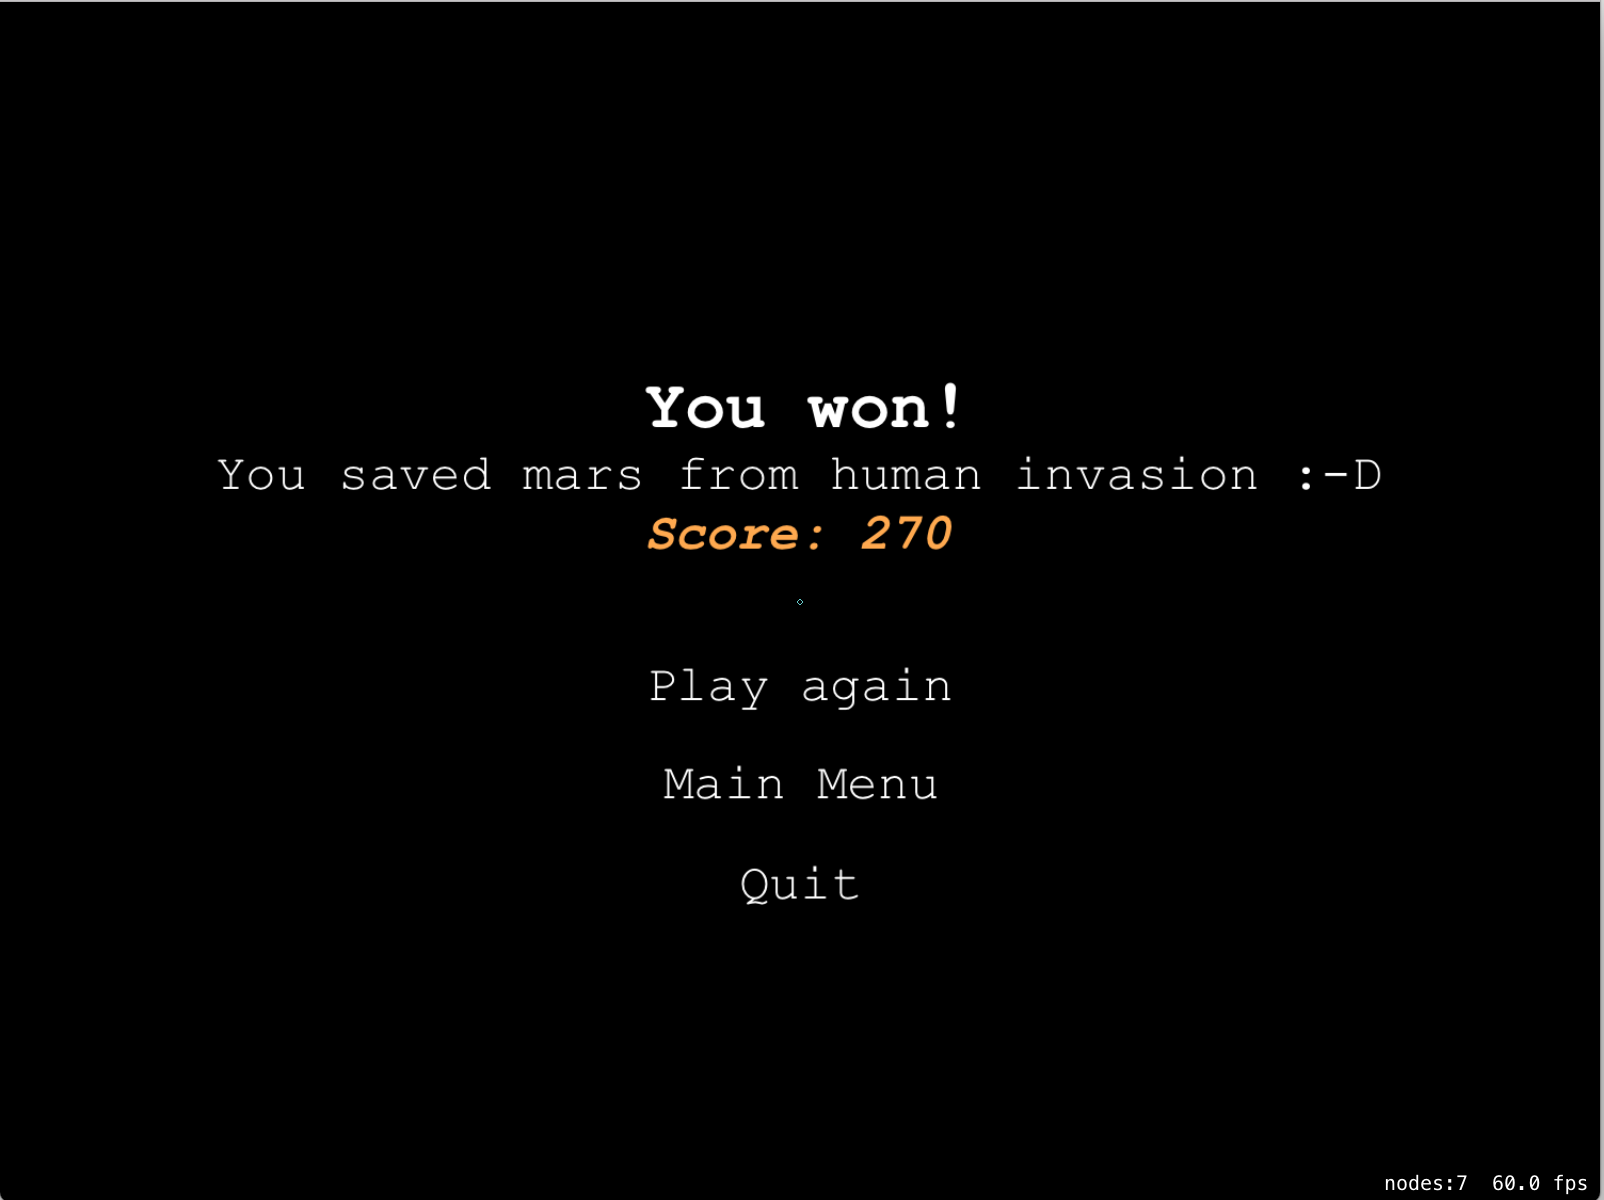
\includegraphics[width=12cm,height=8cm,keepaspectratio]{images/win.png}
    }
    \label{fig:figura1}
\end{figure}

\begin{figure}[htb]
    \centering
    \caption{Final do jogo: derrota}
    \fbox{
        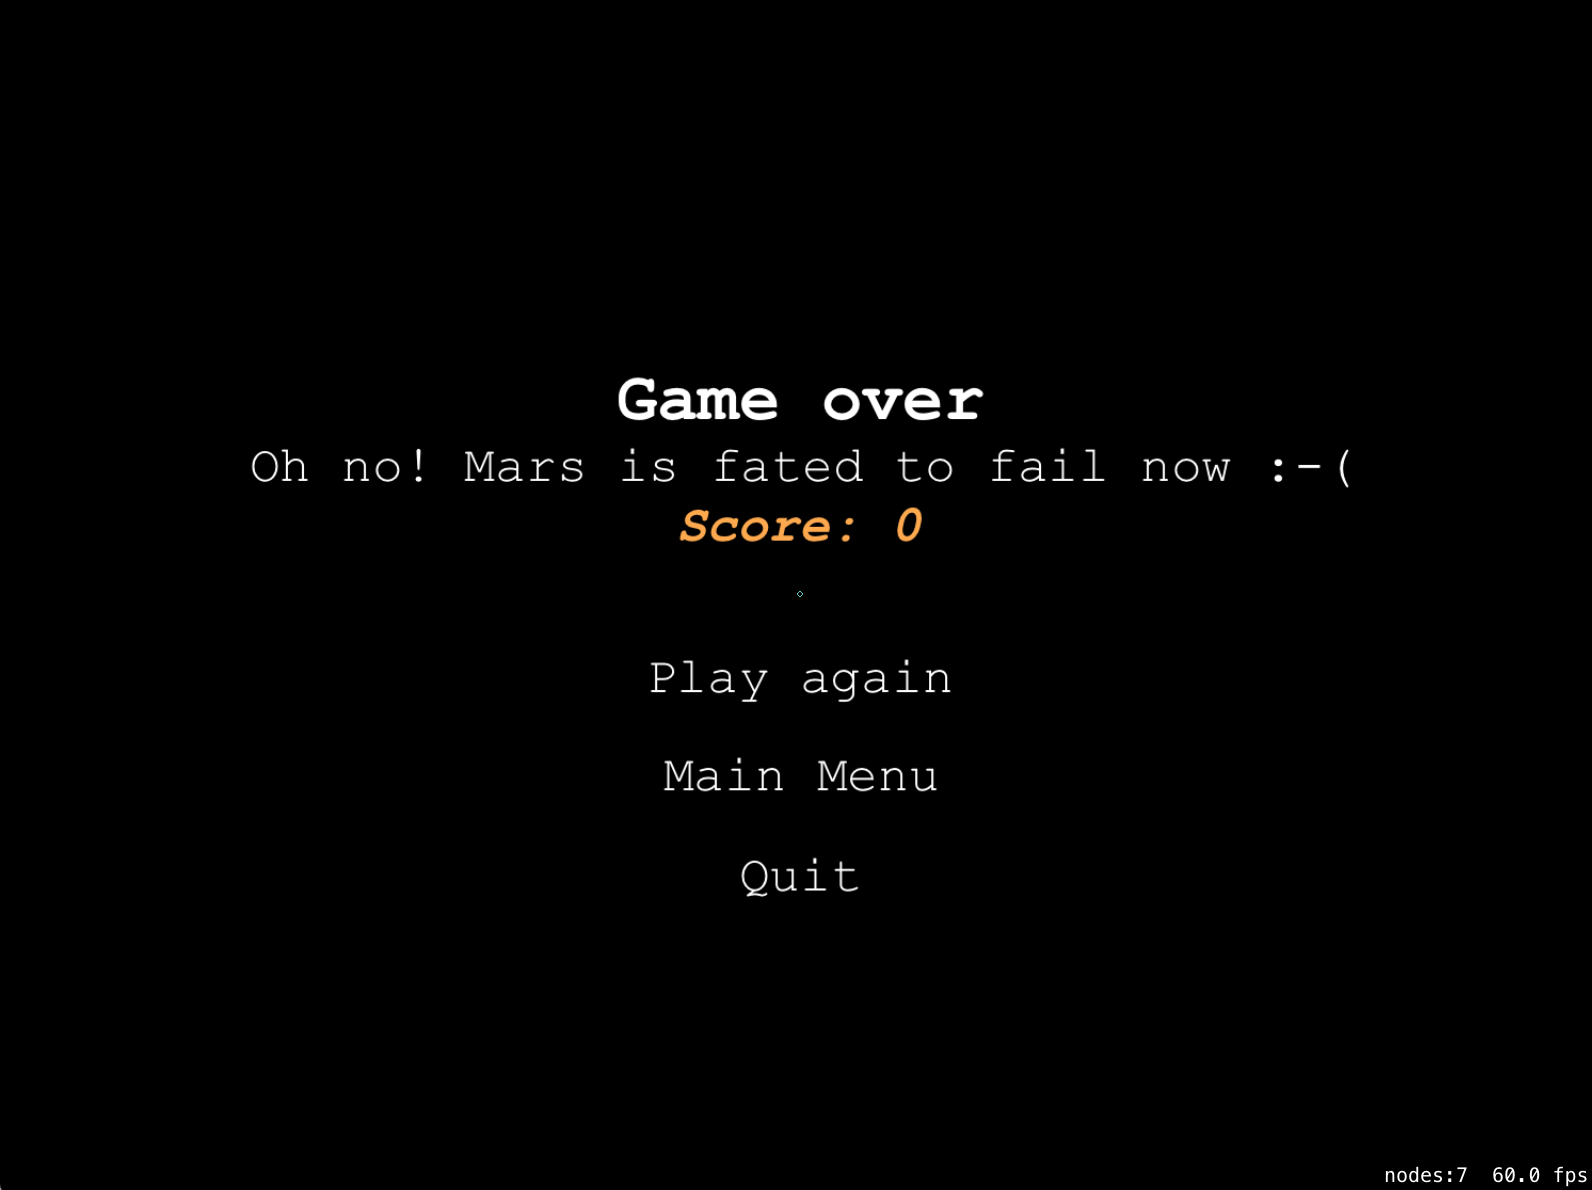
\includegraphics[width=12cm,height=8cm,keepaspectratio]{images/lose.png}
    }
    \label{fig:figura1}
\end{figure}

%%%%%%%%%%%%%%%%%%%%%%%%%%%%%%%%%%%%%%%%%%%%%%%%%%%%%%%%%%%%%%%%%%%%%%%%%%%%%%%%%%%%%
% Conclusão
%
\chapter{CONCLUSÃO}

Ao término do trabalho, podemos concluir que utilizar Orientação a Objetos em projetos que envolvem um grande número de entidades e elementos com diferentes características é muito apropriado.

Isto se deve ao fato de este paradigma se basear na criação de tipos abstratos (com seus atributos e métodos próprios), que permite uma maior separação nas responsabilidades de cada módulo do programa, resultando em um código-fonte mais organizado e conciso.

Já o paradigma funcional não se mostrou tão adequado a um projeto de larga escala com frameworks que dependem de outros paradigmas. Ao menos nossa experiência neste trabalho deixou a impressão de que um projeto grande totalmente funcional não é muito viável.

Entretanto, certos mecanismos associados ao paradigma funcional se mostraram bastante adequados ao projeto, mesmo junto com o uso de orientação a objetos. O uso de funções como \textit{map}, \textit{reduce}, \textit{filter}, e etc reduz a complexidade do código e o torna mais legível e elegante. O mesmo vale para o uso de funções lambda, muito utilizadas em \textit{Javascript} e linguagens de script em geral.

Podemos concluir, por fim, que este trabalho nos auxiliou no aprendizado - através da prática - dos conceitos apresentados em ambos modelos de linguagens de programação (Orientação a Objetos e Funcional) e também na observação dos pontos positivos e negativos de cada um.

%%%%%%%%%%%%%%%%%%%%%%%%%%%%%%%%%%%%%%%%%%%%%%%%%%%%%%%%%%%%%%%%%%%%%%%%%%%%%%%%%%%%%
% Referências
%

%\bibliographystyle{unsrt}
\bibliography{biblio}

\end{document}
